\section{Desarrollo experimental 3}
En este tercer experimento se busca medir la resistencia de un sistema de puesta a tierra, para esto se utilizó un telurímetro UNI-T UT522. El telurímetro esta conformado por una fuente de corriente de baja frecuencia, con una frecuencia diferente a la de la red eléctricapara evitar interferencias, que inyecta corriente entre los dos electrodos auxiliares y un voltímetro que mide la caída de tensión de estos electrodos el cual tiene su lectura calibrada en ohms. 
\subsection{Sistema de puesta a tierra del laboratorio central de electrónica}
En el primer lugar que se realizo la medición fue en el laboratorio central de electrónica, el cual tiene su puesta a tierra accesible a través de una toma de tierra ubicada en la pared. Como no es posible acceder a la malla conductora ubicada debajo del piso se utilizaron dos pesos con una planchas de acero de 20x20cm con un paño muy humedo abajo como electrodos auxiliares, los cuales se colocaron a 10m de distancia entre sí.
\begin{figure}[H]
    \centering
    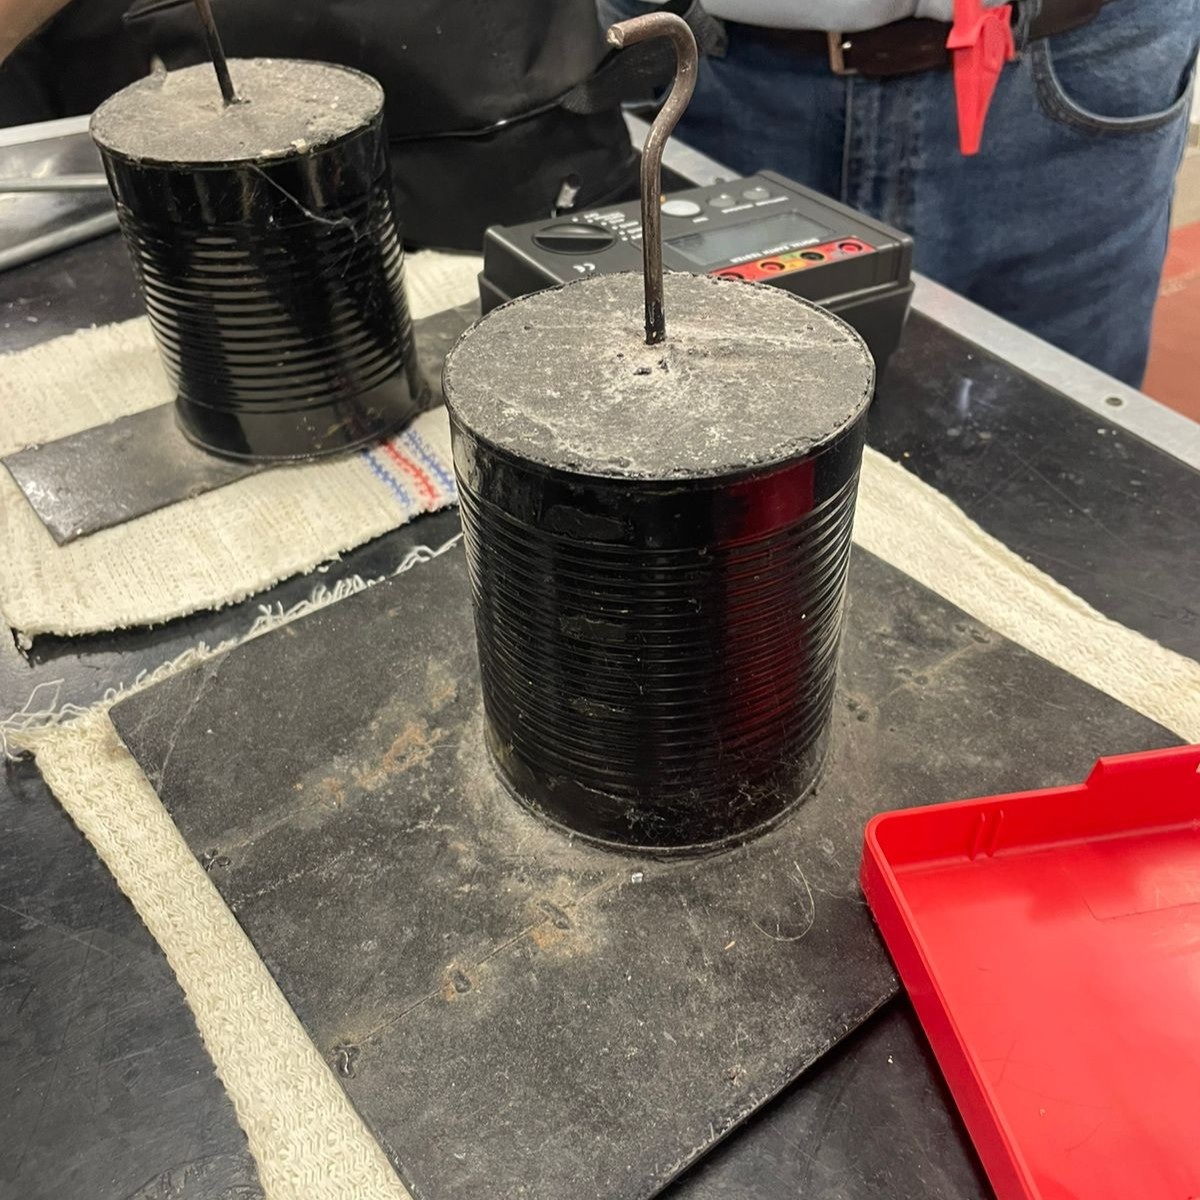
\includegraphics[width=0.5\textwidth]{images/planchas.jpeg}
    \caption{Planchas de acero utilizadas como electrodos auxiliares para la medición de resistencia de puesta a tierra.}
\end{figure}

Una vez colocadas se conectan al telurímetro junto con la puesta a tierra del laboratorio cuidando de que nos se sobrepongan los cables para evitar interferencias por inducción. La puesta a tierra se conecta al terminal \textbf{E} y los electrodos auxiliares al terminal \textbf{P} y \textbf{C}. 

\begin{figure}[H]
    \centering
    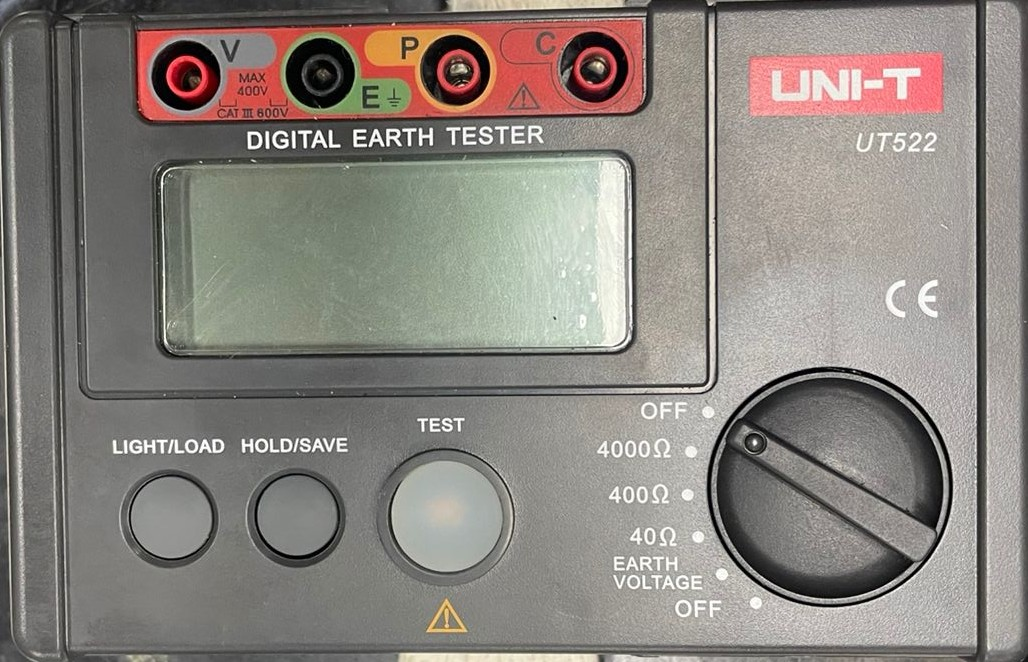
\includegraphics[width=0.5\textwidth]{images/telurimetro.jpeg}
    \caption{Telurímetro utilizado}
\end{figure}

Primero se realizo la medición en el rango de 4000 ohms, obteniendo una lectura de 0.8 ohms, luego al de 400 ohms y por último al rango más adecuado para la medición que es el de 40 ohms, obteniendo en este último una lectura de 0.78 ohms. \\

Una vez medido el sistema de puesta a tierra se verificó que tanto una de las mesas de trabajo como la fuente ubicada en esta estén conectadas a la puesta a tierra. En el caso de la mesa se determinó que esta no estaba conectada a tierra dando una medición de +4000 ohms, mientras que la fuente si estaba conectada a tierra con una medición de 2.2 ohms.

\subsection{Sistema de puesta a tierra fuera del edificio central}
Luego se realizó la medición de la resistencia de puesta a tierra en el exterior del edificio central, para esto se utilizó el mismo método que en el caso anterior pero colocando javalinas en tierra como electrodos auxiliares. En este caso se obtuvo una medición de 0.28 ohms. Se concluyó que es un mejor resultado debido a que se utilizaron electrodos auxiliares directo en tierra y con una mayor superficie de contacto, además las distintas puestas a tierras del edificio que actuan como reisstencias en paralelo.

\subsection{Medición de incertidumbre}

En las especificaciones del telurímetro se indica que en el rango de 40 ohms hay un $\pm 2\%$ de error proporcional de lectura y 20 de error por dígitos menos significativos, como se tienen 2 decimales la resolución es de 0.01 ohms.

\begin{equation*}
\begin{split}
    \Delta R &= R_{medida} \cdot \frac{error_{prop}}{100} + error_{digitos} \\
    \Delta R &= 0.78\Omega \cdot \frac{2}{100} + 20 \cdot 0.01\Omega \\
    \Delta R &= \pm0.2156\Omega
\end{split}
\end{equation*}
Por lo tanto la resistencia de puesta a tierra del laboratorio central de electrónica es de $R_j = 0.78\Omega \pm 0.22\Omega$. \\

En el caso de la medición realizada en el exterior del edificio central, la resistencia de puesta a tierra es de $0.28\Omega$ y se utiliza la misma escala de 40 ohms.
\begin{equation*}
\begin{split}
    \Delta R &= 0.28\Omega \cdot \frac{2}{100} + 20 \cdot 0.01\Omega \\
    \Delta R &= \pm0.2056\Omega
\end{split}
\end{equation*}
Por lo tanto la resistencia de puesta a tierra del laboratorio central de electrónica es de $R_j = 0.28\Omega \pm 0.21\Omega$.